\section{Proposed RRT algorithm}
Rapidly exploring Random Trees (RRTs) where first introduced by Lavalle as a family of randomized planners \cite{LavalleRRT} in 1998. These algorithms are sample based planners. An RRT algorithm grows a tree in the configuration space by randomly sampling configurations and then adding them to the tree. In path planning applications when the algorithm starts the tree contains only the start configuration, the tree is then grown until it contains also the goal configuration. There is a vast set of RRT variations in the literature, an overview won't, however, be presented in this work.
\par
 An RRT which computes paths with a maximum curvature limit is presented. This algorithm was also empowered with the capability to plan in time-dependent environments. In this work, unlike it is done in most of the literature, the sequence of way-points that describe the trajectory is not defined by the vertices of the tree. \textbf{The waypoints are represented by the edges in the trajectory}. The middle point of the edge represents the position, while the alignment of the edge represents the direction of the speed.

\begin{figure}[ht!]
    \centering
    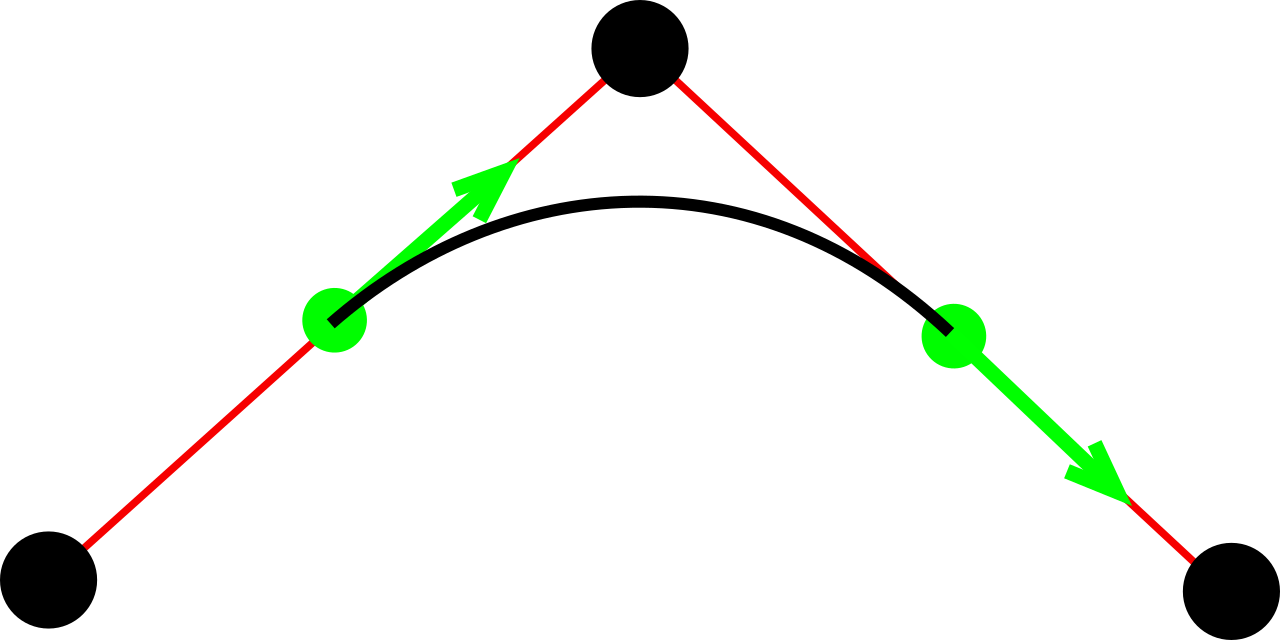
\includegraphics[width=0.4\linewidth]{Figures/04_rrt/waypointsNedges.png}
    \caption{The green points and arrows represent the robot's position and speed respectively. The black points represent the vertices of the RRT.}
    \label{robotStates}
\end{figure}

\subsection{Acceptable angle between edges}
It will now be defined the maximum allowed angle between consecutive edges as a function of the robot minimum curvature radius. Let $d$ be the edge length, $R_{min}$ be the robot minimum curvature radius and $\alpha$ be the angle (maximum angle) between consecutive edges. The angle $\alpha$ will be given in rad as:

\begin{equation}
    \alpha = \pi - 2 * arctan \left ( \frac{R_{min}}{d/2} \right )
\end{equation}

It is obvious that the angle $\alpha$ can only take values between $0$ and $\pi$, in this range the function $cos(\alpha)$ is always decreasing, therefore limiting a maximum angle between two edges is the same as limiting a minimum $cos(\alpha)$. Let now $\vec{e_1}$ represent one edge (position of vertex k minus position of vertex k-1) and  $\vec{e_2}$ represent its consecutive edge (position of vertex k+1 minus position of vertex k). We can state that an edge $\vec{e_2}$ is acceptable after an edge $\vec{e_1}$ if and only if:

\begin{equation}
    \frac{\vec{e_1} \cdot \vec{e_2} }{ |\vec{e_1}| * |\vec{e_2}|} \geq cos(\alpha_{MAX})
    \label{eq:allignable}
\end{equation}

\subsection{Maximum curvature expansion}
Sometimes a new vertex is created in such a position that it is not possible to create an edge from the previous vertex that is aligned with the new vertex (when the condition in equation \ref{eq:allignable} is not respected), such as in Figure \ref{fig:alignable}.



\begin{figure}[ht!]
    \centering
    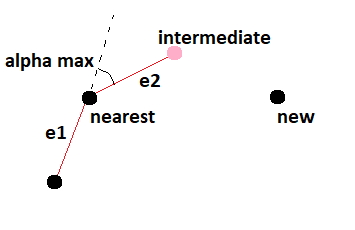
\includegraphics[width=0.6\linewidth]{Figures/04_rrt/alignable.png}
    \caption{The new vertex is in such a position that it is not possible to expand the tree directly towards it, the tree is expanded than using a maximum curvature expansion.}
    \label{fig:alignable}
\end{figure}

In those cases an expansion is made in which the angle between the newly added edge and the edge that leads to that same edge is the maximum allowed angle $\alpha_{MAX}$. In this work this sort of expansion of the tree is called maximum curvature expansion.
\par
 For creating paths that respect the minimum curvature radius constraint, the presented algorithm expands the tree towards the random configurations using successive maximum curvature expansions, until it is possible to expand the tree directly towards the random configuration.

\subsection{Moving obstacles}
To allow this RRT to plan trajectories in environments with moving obstacles a time instant must be associated with each vertex on the tree. For that, each time a vertex is added to the three a time instant is associated with that same vertex. This time-instant is simply the sum of the time-instant associated with the vertex to which the new vertex is connected, plus the distance between these vertexes, divided by the speed of the multi-rotor.

\subsection{Enhancement step}

As it is known trajectories computed by the RRTs might be very sub-optimal. Optimal RRT related algorithms require often great computational times like it was mentioned before. An enhancement step is now proposed. This enhancement step allows the solution computed by the modified RRT to be enhanced in a very significant way without requiring much computational time.
\par
The enhancement step consists in trying, from each vertex in the RRT, to reach directly another vertex, as further in the trajectory as possible. A scheme is now presented in order to demonstrate this concept in Figure \ref{fig:enhancement}:

\begin{figure}[ht!]
    \centering
    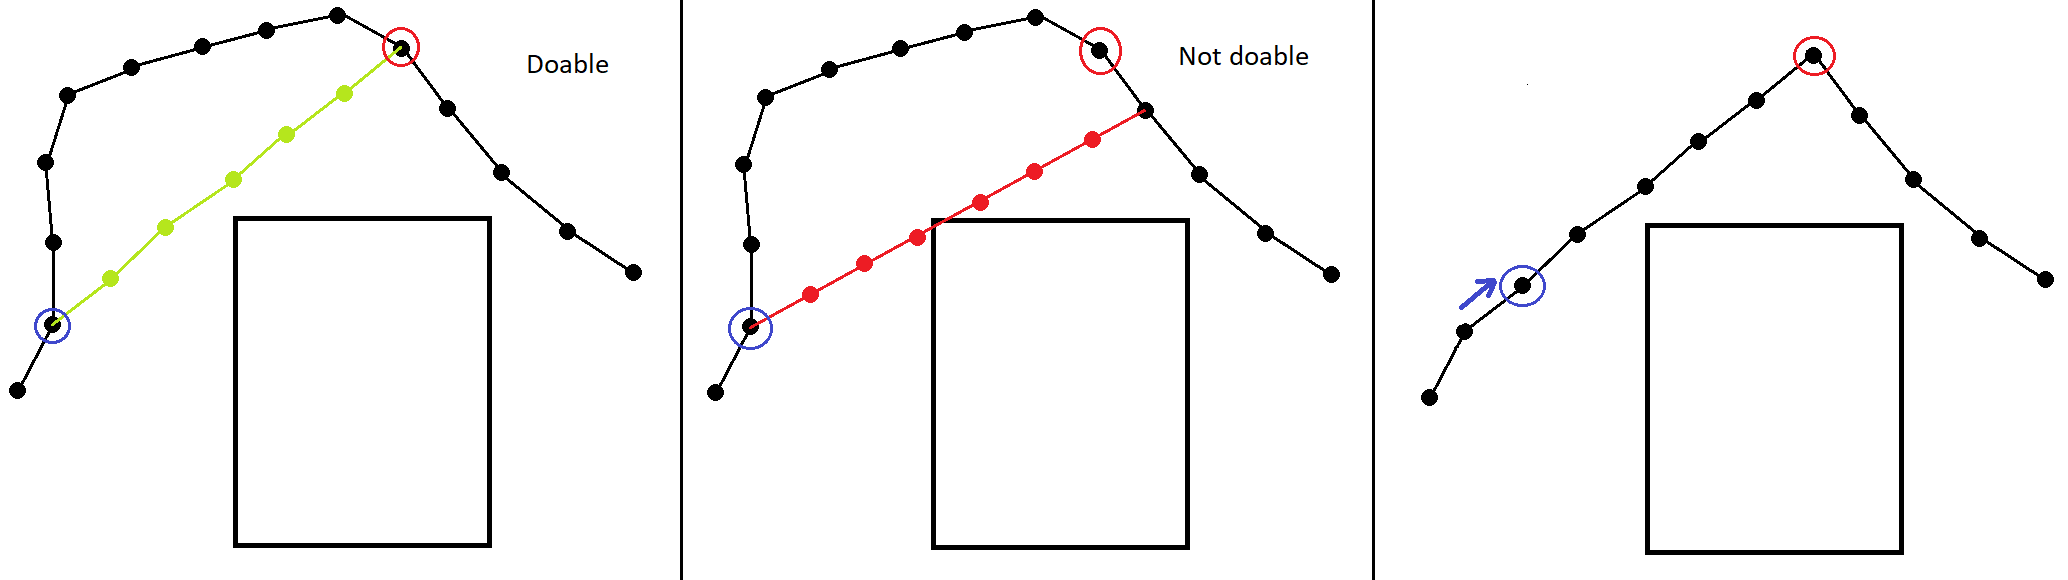
\includegraphics[width=\linewidth]{Figures/04_rrt/REPORTfIGURE.png}
    \caption{Consecutive steps in the enhancement algorithm.}
    \label{fig:enhancement}
\end{figure}

Figures \ref{fig:enhancementRes1} and \ref{fig:enhancementRes2} show some examples of the computed trajectories before and after the enhancement step.

\begin{figure}[ht!]
    \centering
    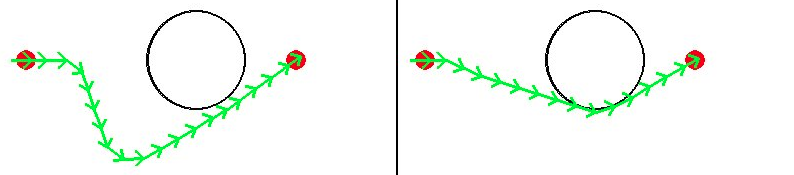
\includegraphics[width=0.6\linewidth]{Figures/04_rrt/result1.png}
    \caption{Example of the trajectory before (on the left) and after (on the right) the trajectory enhancement}
    \label{fig:enhancementRes1}
\end{figure}

\begin{figure}[ht!]
    \centering
    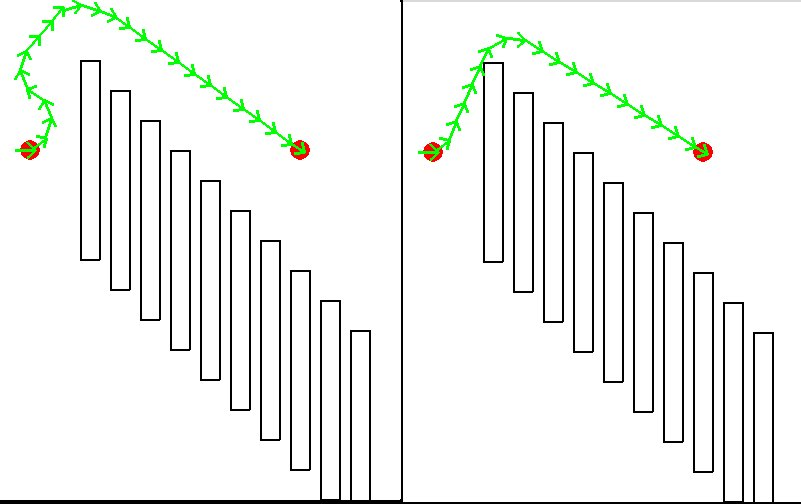
\includegraphics[width=0.6\linewidth]{Figures/04_rrt/result4.jpg}
    \caption{Example of the trajectory before (on the left) and after (on the right) the trajectory enhancement}
    \label{fig:enhancementRes2}
\end{figure}


The algorithms for enhancing the trajectory were performed after growing the RRT 100 times in each environment. Let environment 1 and 2 refer to the environments shown in Fig. \ref{fig:enhancementRes1} and \ref{fig:enhancementRes2} respectively. Let pseudo-sub-optimality (pso) refer to the relation between the trajectory length and the minimum possible length if there were no curvature constraints. The pso is computed using the expression:
$$
pso=\frac{length-optimalLength}{optimalLength} \times 100\%
$$
Where $length$ is the length of the trajectory and $optimalLength$ the length if there was no curvature constraints. The results are presented in Tables \ref{tab:enhancement1} and \ref{tab:enhancement2}:


\begin{table}[ht!]
\begin{tabular}{|l|lll|}
\hline
Env. 1       &  time (s) & length    & pso     \\ \hline
First trajectory    &   0.028   & 474               &  38.6\%                   \\
Enhancement & 0.026  & 376               &  9.64\%                   \\
Final               & 0.054     & 376               &  9.64\%         \\ \hline
\end{tabular}
\caption{Results of the application of the RRT algorithm and enhancement step to environment 1}
\label{tab:enhancement1}
\end{table}

\begin{table}[ht!]
\begin{tabular}{|l|lll|}
\hline
Env. 2       &  time (s) & length & pso \\ \hline
First trajectory    & 0.004     & 435            & 50\%                   \\
Trajectory enhancement & 0.013  & 308            & 6.21\%                 \\
Final               & 0.017     & 308            & 6.21\%                 \\ \hline
\end{tabular}
\caption{Results of the application of the RRT algorithm and enhancement step to environment 2}
\label{tab:enhancement2}
\end{table}

It is possible to observe from Tables \ref{tab:enhancement1} and \ref{tab:enhancement2} that the enhanced trajectories have a length significantly closer to the optimal length.